\documentclass{sig-alternate}
\usepackage{float}
\restylefloat{table}

\title{CSCI-620 Data Management with the IMDb Dataset}
\subtitle{[Understanding, modeling, and developing tools to interact with the IMDb dataset]}
\numberofauthors{4}
\author
{
	\alignauthor
	Aishwarya Rao
	\email{ar2711@rit.edu}
	\alignauthor
	Apurav Khare
	\email{ak2816@rit.edu}
	\and
	\alignauthor
	Martin Qian
	\email{jq3513@rit.edu}
	\alignauthor
	Prateek Kalasannavar
	\email{pk6685@rit.edu}
}

\begin{document}
	\maketitle
	\begin{abstract}
		This project aims to explore a dataset by understanding it, modeling it to a normalized relational schema so that it can be stored and retrieved from a relational database management system. The project also focuses on developing an interface that allows fast and easy access to the dataset by abstracting complex query scenarios, like search by specific parameters within and across tables, and aggregate queries.
	\end{abstract}
	
	\section{Project Status}
	As established in Phase 0, the deliverable of Phase 1 includes an entity-relationship diagram of the IMDb dataset based on our exploration and understanding of the dataset structure. This ER diagram is then used to map to a relational schema. These structures have been designed keeping in mind possible query scenarios, ease of access of writing queries as well as fetching results with respect to common requests, and the constraints required to keep ambiguity and inconsistency out of the structure. 
	\subsection{ER Diagram}
	The ER Diagram representing the design of the database is depicted in Figure \ref{ER}
	\begin{figure}[ht]
		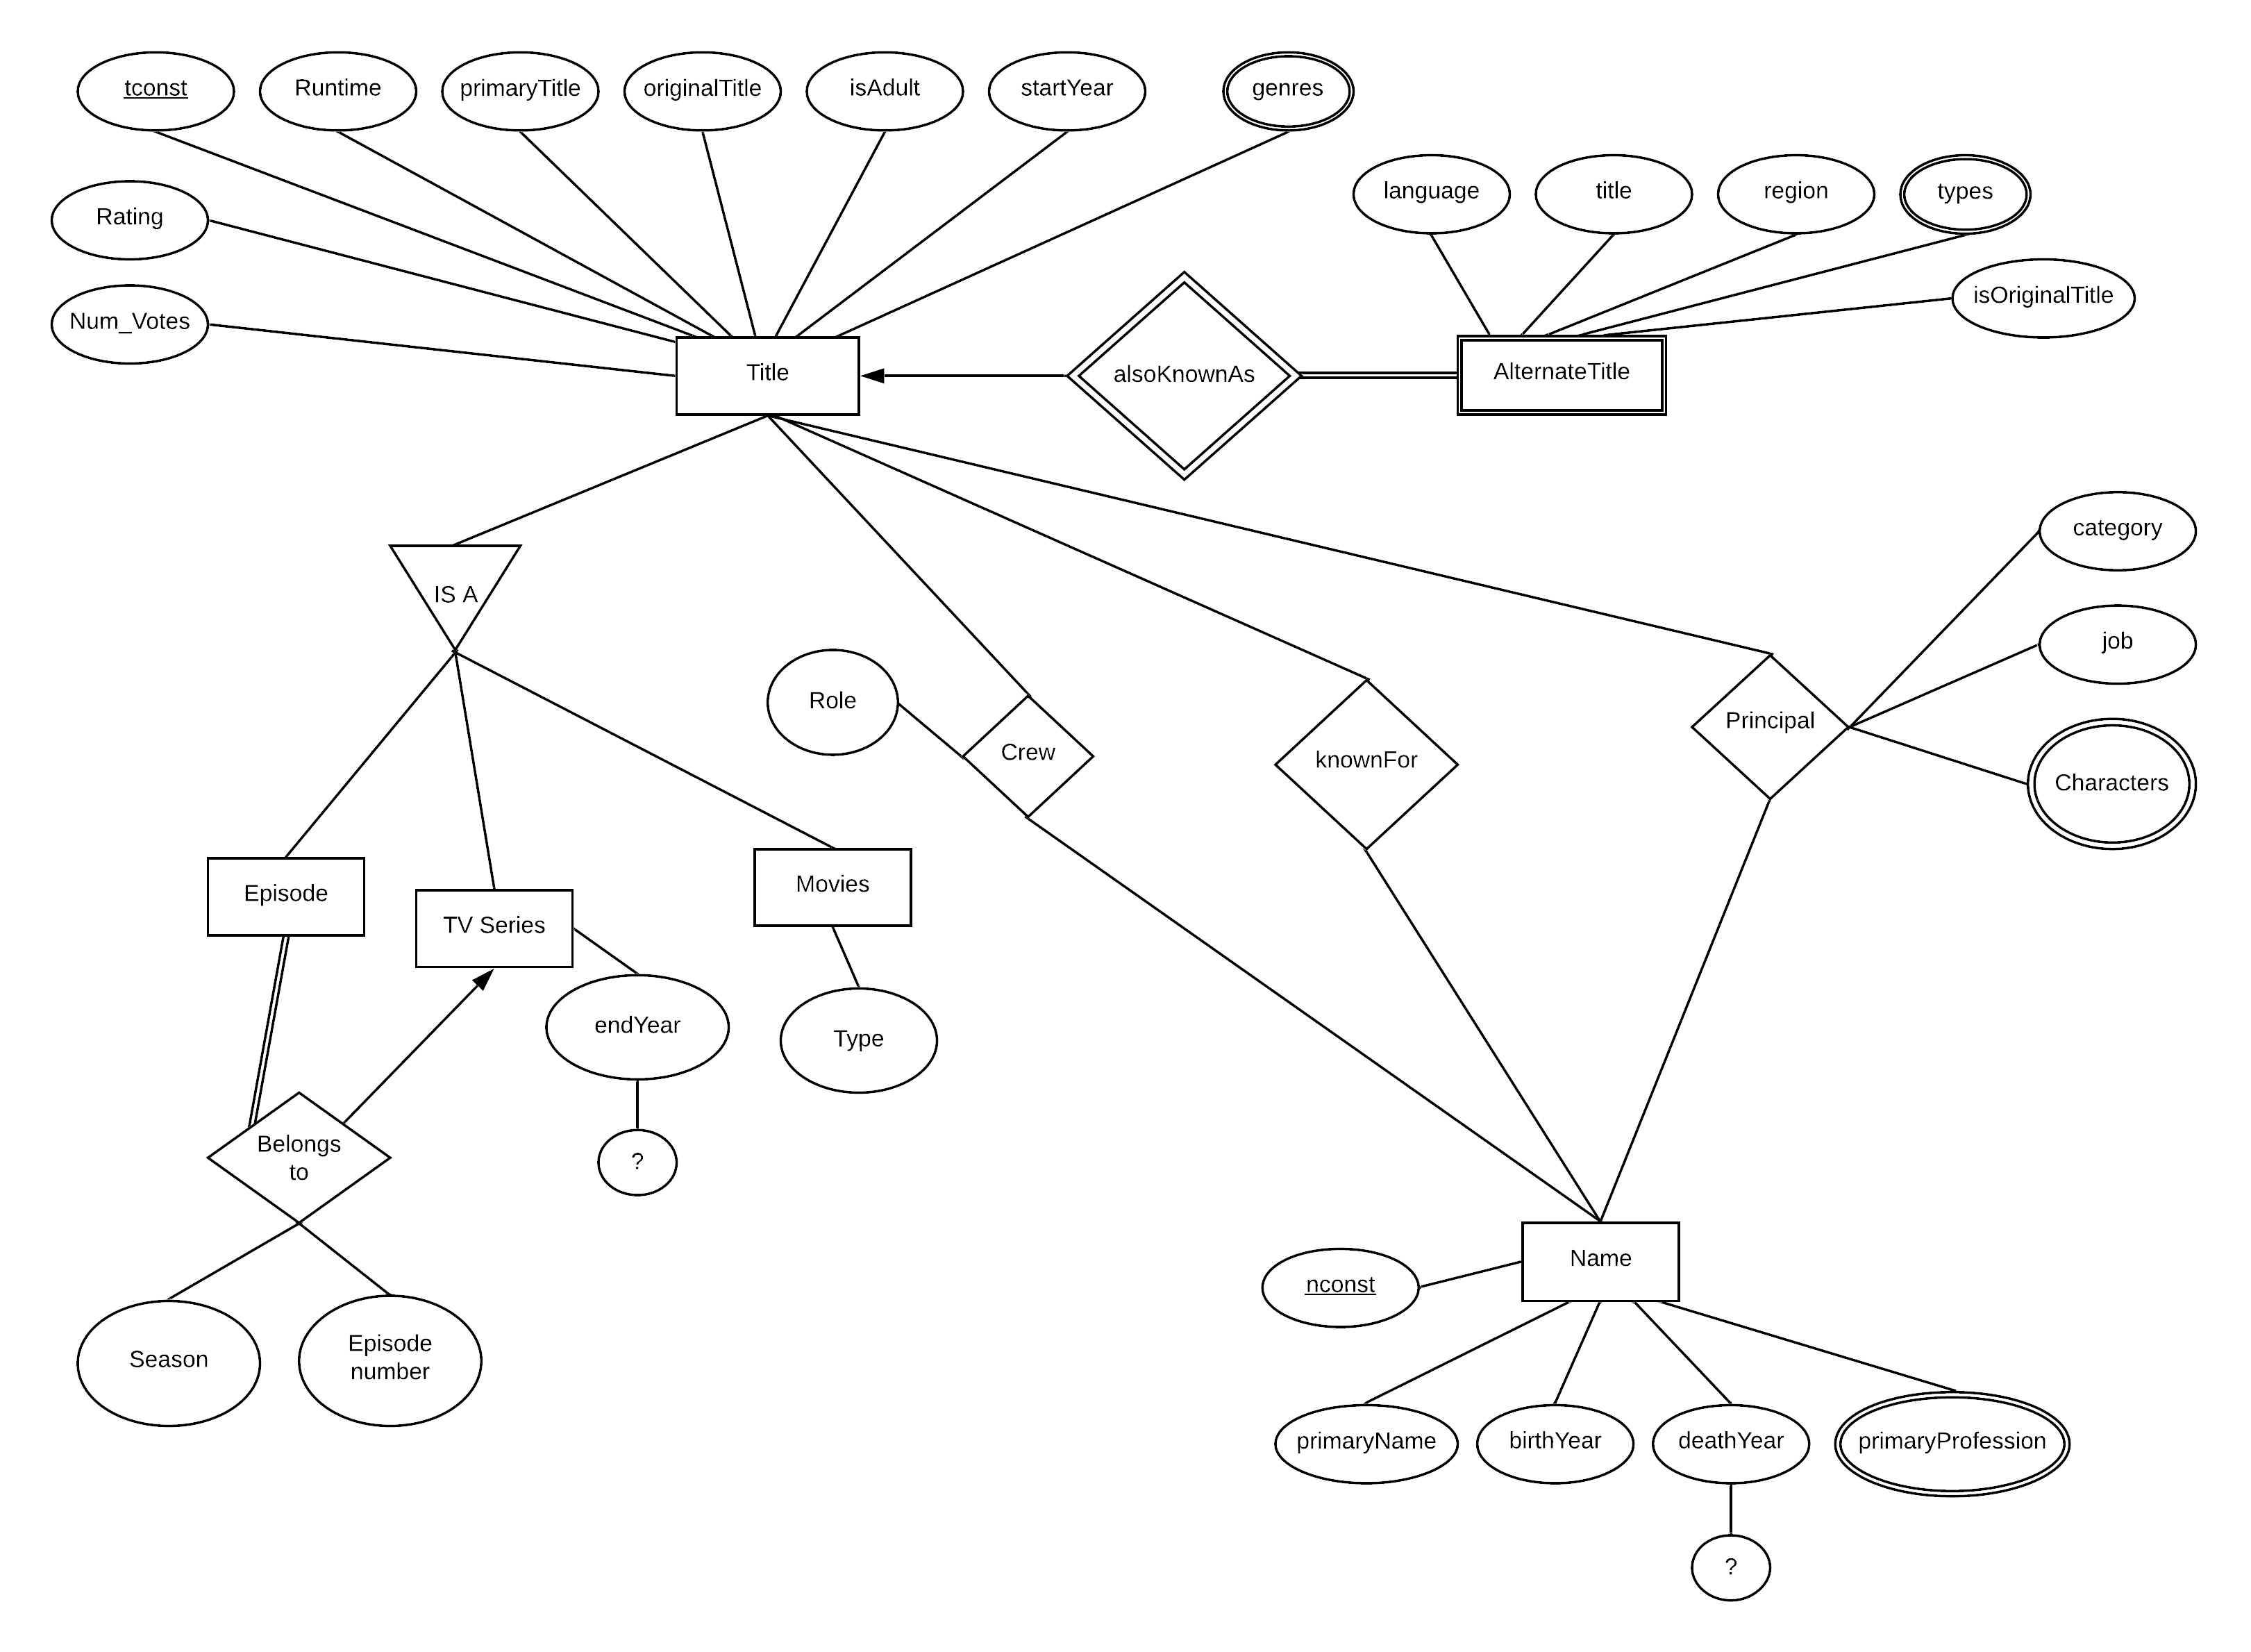
\includegraphics[width=8cm]{er.png}
		\label{ER}
		\centering
	\end{figure}
	The core entity set of the data is the title, which represents a movie or a series or a short. Basic properties that are common among these types are attributes of the title table. To differentiate between movies (which have no episodes) and TV shows, both of whose titles are present in the title table, an IS A relationship is defined. It is assumed that shorts and documentaries are part of movies as they have no separate unique features of their own. Only TV show titles are associated with episode titles with the season and episode number. The rating and the number of votes are considered as attributes of a title since fine-grained information about each review and its rating is not available in the dataset. 
	The other core entity set of the data is the ``name", which refers to the metadata of a person that has participated in a title. Nconst acts as the primary key in this table. 
	A person can have more than one primary profession and hence, this forms a multivalued attribute.
	The relationship between title and a person is in three different forms. One, a person may be a part of the crew for a movie or episode. This job includes producers and writers and are indicated through the role attribute on this relationship. A person may be primarily known for one or more titles. This relationship is captured by known for. Finally, the details regarding the principal team involved in a movie or show (including actors) are represented by a relationship principal that holds the person's role as well as characters they may have played. 
	\subsection{Schema Identification}
	This phase involves the identification and mapping of the relational schema from the entity- relationship Model, as well as choose appropriate constraints and keys required to maintain data integrity and avoid redundancies. The relational schema selected is as follows,\newline
	title (\underline{tconst}, titleType, primaryTitle, originalTitle, isAdult, startYear, averageRating, numVotes)\newline
	title\_genre (\underline{tconst}, \underline{genre}) \newline
	Foreign Key - tconst from title \newline
	tvSeries (\underline{tconst}, endYear)\newline
	Foreign Key - tconst from title\newline
	movie (\underline{tconst}, movieType)\newline
	Foreign Key - tconst from title\newline
	tvEpisode (\underline{tconst}, \underline{parentTconst}, seasonNumber, episodeNumber)\newline
	Foreign key 1 - tconst references title\newline
	Foreign key 2 - parentTconst references tvSeries(tconst)\newline
	alternate\_title (\underline{tconst}, \underline{language}, \underline{title}, \underline{region}, isOriginal) \newline
	Foreign key - tconst references title(tconst)\newline
	alternate\_title\_types (\underline{tconst},\underline{language}, \underline{title}, \underline{region}, \underline{type}) \newline
	Foreign key - tconst references title(tconst)\newline
	name (\underline{nconst}, primaryName, birthYear, deathYear) \newline
	name\_primary\_profession (\underline{nconst}, \underline{primary\_profession}) \newline
	Foreign key - nconst references name(nconst)\newline
	crew (\underline{nconst}, underline{tconst}, underline{role}) \newline
	Foreign key 1 - nconst references name(nconst) \newline
	Foreign key 2 - tconst references title(tconst) \newline
	popular\_titles (\underline{tconst}, \underline{nconst}) \newline
	Foreign key 1 - nconst references name(nconst) \newline
	Foreign key 2 - tconst references title(tconst) \newline
	principal (\underline{tconst}, \underline{nconst}, \underline{category}, \underline{job}) \newline
	Foreign key 1 - nconst references name(nconst) \newline
	Foreign key 2 - tconst references title(tconst) \newline
	principal\_characters (\underline{tconst}, \underline{nconst}, \underline{category}, \underline{job}, \underline{characters}) \newline
	Foreign key 1 - nconst references name(nconst) \newline
	Foreign key 2 - tconst references title(tconst) \newline
	Foreign key 3 - category references principal(category) \newline
	Foreign key 4 - job references principal(job) \newline
	\subsection{Populating the database}
	Python is used to clean up the dataset and prepare it for transfer to a SQL database. SQL scripts are used for creation and insertion of the preprocessed data into the database. These scripts handle the mapping of the original dataset structure and the relational schema.
	Missing values for attributes such as endYear and deathYear are stored as NULL.
	\section{Project outline}
	The next step of the project is to identify possible scenarios and create queries for the same. The query scenarios we forsee implementing include the range of movies during a specified time period, popular movies by a specified actor, top list of movies of all time, specific movie or actor information based on search. Simultaneously, a front end interface will be developed for user-friendly access to the results returned by the queries. The deliverable by the end of this data management project will be the interface that allows users to access and view the data present in the IMDb dataset in a fast and comprehensible way. 
\end{document}